
%(BEGIN_QUESTION)
% Copyright 2015, Tony R. Kuphaldt, released under the Creative Commons Attribution License (v 1.0)
% This means you may do almost anything with this work of mine, so long as you give me proper credit

The following PLC program was written to control the operation of a large electric motor-driven pump.  A variety of ``permissive'' inputs protect the pump from damage under abnormal conditions, and one permissive in particular (``valve open'') will only allow the pump to start up if one of the valves in the piping system is in the full-open position:

$$\includegraphics[width=15.5cm]{i02561x01.eps}$$

Identify the type of contact (either NO or NC) necessary for each of these electrical switch contacts, based on the trip condition (either {\it high} or {\it low}) and how each input is applied in the PLC program:

\begin{itemize}
\item{} Start pushbutton = {\it NO} or {\it NC}? 
\item{} Throttling valve open limit = {\it NO} or {\it NC}? 
\item{} Stop pushbutton = {\it NO} or {\it NC}? 
\item{} High bearing temperature = {\it NO} or {\it NC}? 
\item{} High vibration = {\it NO} or {\it NC}? 
\item{} High motor temperature = {\it NO} or {\it NC}? 
\item{} Low oil pressure = {\it NO} or {\it NC}? 
\end{itemize}

\underbar{file i02561}
%(END_QUESTION)





%(BEGIN_ANSWER)

\begin{itemize}
\item{} Start pushbutton = {\bf NO}
\item{} Throttling valve open limit = {\bf NC}
\item{} Stop pushbutton = {\bf NO}
\item{} High bearing temperature = {\bf NO}
\item{} High vibration = {\bf NC}
\item{} High motor temperature = {\bf NO}
\item{} Low oil pressure = {\bf NO}
\end{itemize}

A helpful problem-solving technique is to first identify the necessary {\it coloring} which will allow the motor to start up and keep running (i.e. the condition of all permissives during correct operating conditions):

$$\includegraphics[width=15.5cm]{i02561x02.eps}$$

Since the motor is controlled by retentive coil instructions (``Set'' and ``Reset''), we know all the permissive contacts on the Reset rung must be uncolored in order for the motor to run.  The normally-closed ``Valve open'' instruction must be colored in order to allow the Start input to latch the Set coil and start the motor.

\vskip 10pt

Once we know this, we may determing the necessary ``normal'' statuses of all permissive switches in order to make their corresponding PLC program contact instructions colored.  A few examples will be given here:

\vskip 10pt

\noindent
{\bf ``Valve open'' limit switch:} The PLC contact instruction for this permissive is normally-closed, which means that PLC input must be de-energized in order to color that contact instruction.  This means the limit switch must be in the open condition when the valve mechanism moves into the switch's sensing range (in the fully-open position), and close when the valve mechanism moves away from the switch.  A limit switch that is closed with nothing near it is a {\bf normally-closed (NC)} limit switch.
\vskip 10pt

\noindent
{\bf Low oil pressure:} The PLC contact instruction for this permissive is normally-closed, which means that PLC input must be energized with electricity in order to maintain that contact instruction in an uncolored state.  This means the low oil pressure switch must be in the closed condition while everything is running as it should (i.e. adequate oil pressure), and open if oil pressure becomes too low.  A pressure switch that is open when pressure is below the trip threshold is a {\bf normally-open (NO)} pressure switch.

\vskip 10pt

\noindent
{\bf High bearing temperature:} The PLC contact instruction for this permissive is normally-open, which means that PLC input must be de-energized in order to maintain that contact instruction in an uncolored state.  This means the high bearing temperature switch must be in the open condition while everything is running as it should (i.e. low bearing temperature), and close if temperature becomes excessive.  A temperature switch that is open when temperature is below the trip threshold is a {\bf normally-open (NO)} temperature switch.

\vskip 10pt

%(END_ANSWER)





%(BEGIN_NOTES)


%INDEX% PLC, relating I/O status to virtual elements 
%INDEX% Switch, ``normal'' status

%(END_NOTES)


